\documentclass[..thesis.tex]{subfiles}


\tikzstyle{component} = [rectangle, rounded corners = 5pt, inner sep  = 5pt, draw=black, text width=2.5cm, text centered]

\tikzstyle{arrow} = [thick,->,>=stealth]

\lstdefinestyle{caml}{
	showstringspaces=false,
        language=Caml,
        literate=
               {->}{$\rightarrow$}{1},
        morekeywords ={module, sig, val, include},
        emph = [1]{int, bool, unit, list, option}, emphstyle=[1]{\textit},
        emph = [2]{varinfo, exp, lval, fundec}, emphstyle=[2]{\underline} 
}






\begin{document}

\toguide{What is the point here?}

In this section, we give an overview  of \textit{Goblint}, a static analyser for detecting data races in C programs with the focus on Linux device drivers that has been developed in the University of Tartu and in the Technical University of Munich for over 10 years \cite{_goblint_????,apinis_frameworks_2014,vojdanivesal_static_2010}.

\toadd{Cite the article written, \sout{doctoral thesis of Kalmer and Vesal, github repo}}

\toask{Should cite something else?}

\toguide{Why are we intrested in Goblint?}

The original work presented in this thesis builds on top of what is done in Goblint. The background information given in this section will hopefully enable the reader to put that in context.

\tosup{So keep in mind that this is the main objective! I will give some comments, but you should also go through each paragraph of this section and ask if it helps provide context to the next section or is just distracting details.}
\todisc{A lot of refactoring, this still relevant?}
\toguide{Okay, got it. So, what is Goblint?}

Goblint is a constraint system based analysis tool that performs abstract interpretation, building on top of the theoretical ideas described in the previous sections. Goblint is written in OCaml and is publicly available on Github.

Goblint takes a C program as an input and uses the CIL framework to process it into an intermediate form that can then be converted into a control flow graph (\textit{CFG}). 

\toadd{cite CIL}

As the next step, the enabled \textit{analyses specifications} are combined and a constraint system that corresponds to the combined analyses and CFG of the program is produced.

The generated constraint system is then solved with a generic constraint system solver. 

Finally, the output is mapped to the original C program and displayed to the user in a suitable format.

\begin{figure}[H]
  \centering
  \begin{tikzpicture}[node distance = 2.5cm and 1.5cm]
    \node (cil) [component] {CIL preprocessor};
    \node (cfg) [component, below of=cil] {control flow graph constructor};
    \node (conssyst) [component, below of = cfg] {constraint system constructor} ;
    \node (analyses) [component, right  =of conssyst] {analyses combiner};
    \node (analysesb) [component, right  =of analyses] {analyses b};
    \node (analysesa) [component, above of = analysesb] {analyses a};
    \node (analysesrest) [component, below of = analysesb] {$\ldots$};
    \node (analyzer) [component, below of = conssyst] {analyzer};
    \node (generic) [component, right  =of analyzer] {generic constraint system solver};
    \node (output) [component, below of = analyzer] {output formatter};

    \draw [arrow] (cil) -- (cfg);
    \draw [arrow] (cfg) -- (conssyst);
    \draw [arrow] (conssyst) -- (analyzer);
    \draw [arrow] (analyzer) -- (output);
    
    \draw [arrow] (analyses) -- (conssyst);
    
    \draw [arrow] (analysesa) -- (analyses);
    \draw [arrow] (analysesb) -- (analyses);
    \draw [arrow] (analysesrest) -- (analyses);

    \draw [arrow] (generic) -- (analyzer);

  \end{tikzpicture}
  \caption{The structure of Goblint}
\end{figure}


\toguide{Okay, do we need to understand all of it?}

The most interesting components of Goblint are the provided solvers for the constraint systems and the wide array of analyses. We will be focusing on the structure of an analysis, using the example of the mutex analysis, which makes use of the previously discussed ideas about lockset analysis. This will hopefully both introduce one of the key analysis for Goblint and give a high-level idea of how an implementation of an analysis looks like. The signatures we introduce are simplified versions of the ones present in the Goblint implementation.

\toadd{\sout{Thesis of Kalmer and Vesal} something else?}
The solvers implemented in Goblint do not fall with the scope of this thesis. A thorough overview can be found from \cite{apinis_frameworks_2014, vojdanivesal_static_2010}.

\toguide{So, how does an analyses look like?}

As previously described, for each analysis, we need an abstract domain to perform the abstract interpretation on. In Goblint, all the domains implement interface \inlinecode{Lattice}. The functions \textit{join} and \textit{meet} correspond to the binary least upper bound and greatest lower bound operations. 


\begin{lstlisting}[language=Caml,style=caml]
module type Lattice =
sig
  type t
  val leq: t -> t -> bool
  val join: t -> t -> t
  val meet: t -> t -> t
  val bot: unit -> t
  val is_bot: t -> bool
  val top: unit -> t
  val is_top: t -> bool
  ...
end
\end{lstlisting}

The type \inlinecode{t} in OCaml module type leaves the type abstract. From here on, the types written in italics are built-in types in OCaml. 

\tosup{\sout{I would not talk about Printable, so I suggest just inlining the type t into the Lattice. Maybe also remove is\_top \& is\_bot. Say somewhere on top that these are simplified/partial signatures.}}


In case of the lockset analysis, the domain is a reversed set domain of all the possible locks. That is, the elements in the domain are sets of locks in the program under analysis and join operation is defined as the intersection of two sets and meet as union of two sets. The reasoning behind the set domain being reversed is that we are interested in the set of all the locks that must be held at a specific statement. In the situation where we have to take an upper bound of the two locksets (say, after two branches of an if-else statement merge), we hence want it to only consist of locks that were in both of the locksets.

Analysis in Goblint must implement the module type \inlinecode{Spec}. Following is the simplified version of it.

\toask{Did I not cover something important? Or something left is maybe not important in context of thesis? Left out: sync, intrpt, }
\toans{No, and I think you can remove more, such as exitstate \& otherstate, but this signature seems okay to me.}

\begin{lstlisting}[language=Caml,style=caml]
module type Spec =
sig
  module D : Lattice
  module G : Lattice

  val name : string

  val startstate : varinfo -> D.t
  val exitstate  : varinfo -> D.t
  val otherstate : varinfo -> D.t

  val part_access: (D.t, G.t) ctx -> exp -> varinfo option -> bool -> (Access.LSSSet.t * Access.LSSet.t)

  val query : (D.t, G.t) ctx -> Queries.t -> Queries.Result.t

  val assign: (D.t, G.t) ctx -> lval -> exp -> D.t
  val branch: (D.t, G.t) ctx -> exp -> bool -> D.t
  val body  : (D.t, G.t) ctx -> fundec -> D.t
  val return: (D.t, G.t) ctx -> exp option  -> fundec -> D.t

  val special : (D.t, G.t) ctx -> lval option -> varinfo -> exp list -> D.t

  val enter   : (D.t, G.t) ctx -> lval option -> varinfo -> exp list -> (D.t * D.t) list
  val combine : (D.t, G.t) ctx -> lval option -> exp -> varinfo -> exp list -> D.t -> D.t

  ...

end
\end{lstlisting}

Here the underscored types are the ones defined in the CIL library.

Each analysis includes two lattices, lattice $D$ will contain the abstract states and lattice $G$ the abstract values for global variables.

The type \inlinecode{ctx} with type parameters $\lp D.t, G.t \rp$ encapsulates both the local and the global state, offering access to helper functions on them. 

The functions \inlinecode{startstate},\inlinecode{exitstate} and \inlinecode{otherstate} provide an initial abstract state for a thread depending on whether the thread starts an
initialization function (in the context of device drivers, the function that registers the driver and exposes the callback functions),
a cleanup function (where deregistration happens in device drivers) or is any other function that can be used to spawn a new thread (all the file operations).

The functions take as argument information about the function declaration, enabling Goblint to differentiate between different file operations.
In case of mutex analysis, all the functions always return empty locksets.

The \inlinecode{part\_access} function enables one to partition accesses into disjoint groups -- if two accesses to the variable $x$ are in different partitions, then they cannot race. In addition, it also associates a set of locks held with the partition. This function makes it possible to use the idea of dividing access information to the left and right side.

In case of the mutex analysis, this function returns empty sets, as it does not make use of partitioning, but plays an important role in region analysis.

\tosup{This function is important and maybe deserves more explanations, or you should at least highlight (forward-ref perhaps) that this function is what you had to interface with and plays an important role for this thesis.}
\todisc{Can backwards ref now :), tied it with the left-hand right-hand side of the last section, anything else? }

The \inlinecode{query} function enables the communication between different analyses that have been combined into one and are being performed at the same time -- 
an analysis must be able to answer the query based on the current context. This allows an analysis to avoid duplication and allows one to design more modular analyses consisting of sub-analyses. More information regarding the query system of Goblint can be found here \toadd{Cite Kalmer}.

The functions \inlinecode{assign}, \inlinecode{branch}, \inlinecode{body} and \inlinecode{return} are functions from abstract state to abstract state, for assignment statements,
branching statements and for entering and exiting from function calls. They correspond to the $\lllb s \rrrb^{*}$ family of functions previously introduced.

In the implementation of mutex analysis, those transfer functions do not actually change the abstract state, as none of the statements influence the set of held locks.
However, they do register accesses to variables, for example, an access is registered for both the left and right hand side of an assignment with further distinction
that the access to the left hand side is a write access.

The \inlinecode{special} function handles functions for which the source code is not available for Goblint to analyse. In the mutex analysis,
this function modifies the abstract state -- function calls to functions such as \inlinecode{\_\_raw\_lock\_unlock} and \inlinecode{\_lock\_kernel} 
remove and add mutexes to the set of held locks.

\toadd{Enter and combine, makes sense if I had this to theoretical part as well. Big if.}

\toguide{Okay, pretty dense stuff.}
\tosup{\sout{This is a pretty big shift in tone from internals to a conceptual description of the analysis. I think both are needed, but it's pretty bad structurally. I might even suggest merging region analysis with your conceptual description of your own contribution and put all implementation details after that chapter where you describe goblint as is and show what changes you made.}}
\todisc{Refactored}

\kalmer{See super-tehniline värk ei huvita kedagi --- siit võib julgelt veel kustutada. Aga suurim probleem on see, et see ei vii kuhugi (peale kokkuvõtte). Siin võiks olla ühe päris näite läbi-mängimine. }

\subsection{Changes}
\toask{Divide this section into two (what is Goblint? My changes and their effect.) or create one more section?}


As part of this thesis, the region analysis was extended to include the time dimension in addition.

A new concurrency domain was added that improves the way Goblint handles detection of processes that are guaranteed to run only in one thread at a time.
A way to append the time partition information to the left side of the access was added with a method to transform the time partition that can be used inside transfer functions. 

The implementation makes vast use of the \inlinecode{part\_access} method. A remaining technical difficulty is that the concurrency domain is ingrained in the base analysis,
one of the oldest analysis in Goblint, and Goblint does not have a preproccessing phase. Therefore, the complexity added to the already complex base analysis is quite extensive.

I hope to solve this issue before requesting the changes to be merged into the mainline.
Meanwhile, a fork of Goblint containing these changes is available here: \url{https://github.com/vootelerotov/goblint-fork}

\toask{How does this seem? Would work on making a decent pull request after turning in the thesis, hopefully something to add to the presentation slides? Alternative would be to focus on the implementation until deadline, but paper still looks raw.}

\toguide{Any effect?}

\subsubsection{Concrete example}

For a concrete example, lets consider following device driver:

\begin{lstlisting}[language=c,style=def,columns=fullflexible]
pthread_mutex_t open = PTHREAD_MUTEX_INITIALIZER;
pthread_mutex_t close = PTHREAD_MUTEX_INITIALIZER;

static int file_open(struct inode *inode, struct file *file)
{
  pthread_mutex_lock(&open);
  file->private_data=1; 
  pthread_mutex_lock(&open);
  return 0;
}

static int file_release(struct inode *inode, struct file *file)
{
  pthread_mutex_lock(&close);
  file->private_data=NULL; 
  pthread_mutex_lock(&close);
  return 0;
}

...
\end{lstlisting}

Previously, Goblint would have seen \inlinecode{private\_data} of \inlinecode{file} as unsafe. At the same time, Linux kernel guarantees that a file cannot be released until it has been opened and it can be opened again only after it has been released. This guarantee has been incorporated into Goblint by partitioning the time for file argument into partitions \textit{fileOpen},\textit{fileClose} and \textit{default}. 

Thanks to this Goblint is able to rule out a possible data race and deem the location to be safe as can been seen from the Goblint output on Figure \ref{Goblint-example}

\begin{figure}[H]
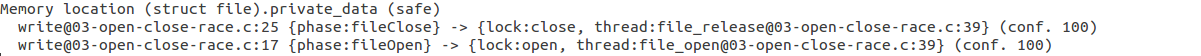
\includegraphics[width=0.9\textwidth]{goblint-out}
\caption{Snippet from Goblint output}
\label{Goblint-example}
\end{figure}
\subsubsection{Evaluation}


Evaluating the effect of the enhanced region analysis on the set of character devices used as benchmark suit for Goblint gave the following results.


\begin{figure}[H]
 \label{evaluation}
 \centering
 \begin{tabular}{|c|c c | c c| }
   \hline
   \multicolumn{5}{ |c| }{Benchmark suite} \\
   \hline
   &  \multicolumn{2}{c}{Indirect races} & \multicolumn{2}{|c |}{Direct races} \\
   Driver & Region  & Enhanched Region  & Region  & Enhanched Region \\ 
   \hline
    apm-emulation.c & 27 & 27 & 24 & 19 \\
    applicom.c & 16 & 15 & 8 & 7 \\
    bsr.c & 19 & 0 & 10 & 2 \\
    dtlk.c & 30 & 23 & 19 & 19 \\
    efirtc.c & 0 & 0 & 0 & 0 \\
    genrtc.c & 0 & 0 & 2 & 2 \\
    hangcheck-timer.c & 12 & 12 & 0 & 0 \\
    hpet.c & 292 & 133 & 27 & 25 \\
    ipmi\_devintf.c & 197 & 117 & 8 & 8 \\
    ipmi\_msghandler.c & 481 & 481 & 273 & 273 \\
    ipmi\_poweroff.c & 142 & 50 & 11 & 11 \\
    ipmi\_watchdog.c & 245 & 224 & 13 & 13 \\
    lp.c & 85 & 85 & 8 & 8 \\
    mem.c & 0 & 0 & 5 & 5 \\
    misc.c & 6 & 6 & 10 & 9 \\
    nvram.c & 0 & 0 & 1 & 1 \\
    pc8736x\_gpio.c & 195 & 0 & 2 & 2 \\
    ppdev.c & 129 & 122 & 14 & 14 \\
    random.c & 65 & 65 & 40 & 40 \\
    raw.c & 264 & 0 & 3 & 2 \\
    rtc.c & 20 & 1 & 4 & 3 \\
    scx200\_gpio.c & 188 & 0 & 1 & 1 \\
    tlclk.c & 86 & 18 & 8 & 7 \\
    toshiba.c & 0 & 0 & 0 & 0 \\
    ttyprintk.c & 193 & 193 & 3 & 3 \\
   \hline
\end{tabular}
\caption{Results of benchmarking region analysis with and without time partitioning}
\end{figure}

We divide the potential data races into two categories. We say that the potential race is \textit{direct} if Goblint deems it unsafe based on the direct access present in the source code
Goblint is analysing. For example, the direct access could be a variable assignment.
An \textit{indirect race} is reported when there is a possibility of a race at a location, when one considers functions for what Goblint does not have the source code for.
This can happen if driver exposes some of its states using a function defined in the Linux kernel.   

In the Figure \ref{evaluation} the columns denoted as \textit{Region} contain results of the analysis of the benchmark suite performed by Goblint with the space based region analysis active, while the column denoted as \textit{Enhanched Region} are results that were achieved by additionally adding the time partitioning. The numbers indicate real data races or false-positives found by Goblint.

As seen by the results of the benchmark, the effect the time partition added to the region analysis depends heavily on the driver.In some drivers it enables Goblint to deem quite a lot of previously unsafe locations to be safe, lessening the amount of false-positives.

In most of the drivers, the positive effect can be attributed to the exclusion of races between \inlinecode{init} and \inlinecode{exit} functions. 

It is worth noting that the motivation for introducing the partitioning by time to Goblint came from analysing the common issues on a subset of those very same drivers.
However, the fact that there were other drivers, outside the subset of the benchmark drivers that were manually analysed
that benefited from the addition of the extra dimension, leads the author to believe that there is a reasonable likelihood
that the benefits are not limited to this specific set of drivers.

\toguide{Okay, got it. Seems cool. Anything else we should know?}

\toask{Leave out?}

The examples given for guarantees were all specific to Linux device drivers and as such, required domain knowledge to specify. This is an hindrance,
specially taking into account that the number of possible conventions that guarantee race freedom between two operations is very likely large.  

However, at the same time it is very hard to imagine a domain independent analysis that would be able to safely exclude the races that we have looked at in this section.

Currently, the rules mentioned in this section are hard-coded into Goblint. This approach does not completely solve the issue of how to make Goblint take the domain specific happen-before
guarantees into account -- sadly it is not possible for the team behind Goblint to cover all the possible domains nor even fully cover the domain of device drivers.

In the long term, offering either the user of a Goblint or an interested thirty party a way to specify those guarantees,
for example through a DSL,  would help to solve this limitation. In addition, an approach that would try to deduce possible happens-before guarantees dynamically 
could be something that would lessen the burden on the party specifying the guarantees.

\toadd{Some kind of ending}
\tosup{It would be nice to have some words about how this is implemented in slightly more low-level terms.}
\todisc{Added above}

\end{document}
